% case overview

\section{Introduction}

The previous chapter explained the methodology used to gather and analyse data for this case-based study. This chapter introduces the three open innovation projects or cases recruited for this study. Each case description includes a brief outline of the main innovation challenge, summary information about the partner organisations and their employees directly involved in the open innovation project, and a statement of progress at the time of data collection. Cases are then compared and contrasted to highlight key differences between them. The reader should have a clear understanding of each open innovation case by the end of this chapter. Names have been altered and geographic places suppressed, not only to protect the identity of organisations and people involved, but also to hide the markets the organisations operate in. \medskip

\section{Case One: Cold chain innovation}

\enquote{Herbs \& More} is a family-owned business that grows and supplies a range of green leaf vegetable products to caterers, restaurants, green grocers and supermarket chains. Products are supplied in bulk or in pre-packaged bags sold by the carton. The pre-packaged bags are supplied either as their own branded product or as a supermarket private-label product. \enquote{Herbs \& More} is based in a region that enjoys a temperate climate, enabling them to grow a greater variety of green leafy vegetables all year round. \enquote{Herbs \& More} competes with a handful of other firms for supply contracts with national supermarket chains. It views itself as a progressive business that combines innovation, expertise, and a good work ethic to provide the highest quality fresh produce to its customers.\medskip

\subsection{Innovation challenge}

Green leaf vegetable products have a shelf-life of eight days post-production. To maximise shelf-life, \enquote{Herbs \& More} have to deliver products by refrigerated trucks to customers in different parts of the country within two to three days of harvesting. Cartons are packed on wooden pallets stacked in two rows down the length of the refrigerated compartment. Maintaining uniform air temperatures between 1\si{\degree}C and 4\si{\degree}C in tightly-packed trucks is challenging. Refrigerated air tends to flows around the outside of a load and not through the load resulting in an uneven temperature distribution, which can lead to spoilage. \enquote{Herbs \& More} have initiated a program to improve on-farm product handling and packaging practices in an effort to reduce spoilage and improve the shelf-life of their products. The cold chain initiative is being driven by the general manager responsible for product processing and delivery at \enquote{Herbs \& More}. His goal is to ensure \enquote{Herbs \& More} is at the forefront of current best practice. \enquote{Herbs \& More} has excellent working relations with its freight forwarders, all of whom are keen to help the company improve on-farm product handling and packaging practices. The freight forwarders have a wealth of experience in cold chain logistics and are motivated to help \enquote{Herbs \& More} in order to maintain goodwill and avoid being penalised when products get rejected because of temperature issues. It is not always clear if rejections are a result of poor on-farm practices or because air temperatures were not properly maintained during transit. Working together and sharing practical knowledge is in everybody's best interest.\medskip

\enquote{Herbs \& More} uses advanced wireless micro-sensor technology provided by \enquote{Keep Fresh} to gain insight into air temperature variation inside loaded trucks. \enquote{Keep Fresh} is a foreign-based firm that specialises in monitoring the condition of perishable goods through the supply chain. They develop, manufacture, and sell miniaturised wireless sensor devices that can be placed inside individual food packages. Each device records time and temperature on a continuous basis for up to 30 days. Data can be retrieved from each device using wireless data readers up to 100m away and uploaded to a central database, where it can be queried in a variety of ways. \enquote{Keep Fresh} is helping \enquote{Herbs \& More} develop an independent monitoring system to identify problem shipments before they are unloaded. \enquote{Herbs & More} have also enlisted \enquote{State University} to model temperature distributions inside refrigerated trucks using the data provided by the wireless sensor devices. \enquote{State University} recently established a research group to investigate how sensor technology and data analytics can be combined to solve practical problems in perishable goods supply chains. \enquote{Herbs & More} hope the modelling done by the research group will lead to better load configurations and packaging material to improve product performance. The cold chain initiative is a good example of inbound open innovation. \enquote{Herbs & More} see this initiative as their first serious foray into open innovation and are keen to improve their knowledge sharing practices. \medskip

The cold chain initiative involves both process and product performance innovation. Because the aim is to improve on-farm product handling and packaging practices, this case may be considered an example of \enquote{incremental innovation} \citep{henderson1990architectural}. \medskip

\subsection{Progress to date}

Case One was still at an early stage at the time of data collection. Some progress had been made collecting temperature data inside refrigerated trucks. Modelling of air temperature distribution was about to commence.. 

\subsection{Participants}

Table \ref{c1_participants} lists the partner organisations involved in Case One. Eighteen people from seven organisations were involved in this case. All 18 people completed the online survey, six of whom were subsequently interviewed. Of the individual participants, only two were female. \medskip

\begin{table}[]
\centering
\caption{Participants - Cold chain innovation}
\label{c1_participants}
\begin{adjustbox}{width=\textwidth}
\begin{tabular}{@{}lllll@{}}
\toprule
\multicolumn{1}{c}{Partner} & \multicolumn{1}{c}{Psuedonym} & \multicolumn{1}{c}{Business focus} & \multicolumn{1}{p{2cm}}{\centering Individual \\ participants} & \multicolumn{1}{p{2cm}}{\centering Number \\ interviewed} \\ \midrule
\multicolumn{1}{c}{1} & "Herbs \& More" & Grow and sell green leafy vegetable products & \multicolumn{1}{c}{6} & \multicolumn{1}{c}{2} \\
\multicolumn{1}{c}{2} & "Cool Transport" & Refrigerated transport and warehousing & \multicolumn{1}{c}{3} & \multicolumn{1}{c}{1} \\
\multicolumn{1}{c}{3} & "Fast \& Fresh" & Refrigerated transport and warehousing & \multicolumn{1}{c}{1} & \multicolumn{1}{c}{0} \\
\multicolumn{1}{c}{4} & "Keep Fresh" & Manufacture and sell cold-chain monitoring technology & \multicolumn{1}{c}{1} & \multicolumn{1}{c}{1} \\
\multicolumn{1}{c}{5} & "Polar Express" & Refrigerated transport and warehousing & \multicolumn{1}{c}{2} & \multicolumn{1}{c}{0} \\
\multicolumn{1}{c}{6} & "Cold Chain Solutions" & Refrigerated transport and warehousing & \multicolumn{1}{c}{1} & \multicolumn{1}{c}{0} \\
\multicolumn{1}{c}{7} & "State University" & Higher education, basic and applied research & \multicolumn{1}{c}{4} & \multicolumn{1}{c}{2} \\ \cline{4-5}
 &  & \multicolumn{1}{r}{Total} & \multicolumn{1}{c}{18} & \multicolumn{1}{c}{6} \\ \bottomrule
\end{tabular}
\end{adjustbox}
\end{table}

Figure \ref{fig:demographics} illustrates key demographic features of individual participants in all three cases. For Case One, the education level of individuals ranges from high-school (secondary) level to doctoral level. Many of the participants have tertiary qualifications. Their educational backgrounds are quite diverse, with participants having qualifications in management and commerce, engineering and related studies, mixed field programmes, agriculture and environmental studies, natural and physical sciences, and education. Participant ages ranged from 27 to 62 years (median age was 47 years). Relevant work experience ranged from 1 to 25 years (median work experience was 9 years). Current job tenure ranged from 1 to 20 years (median job tenure was 7.5 years). \medskip

Figure \ref{fig:proximity_c1} depicts the spherical distance\footnote{Spherical distance is the shortest distance between two points on the surface of a sphere, measured along the surface of the sphere. Distances were calculated using individual work-place postcodes as a geographic reference.} between every individual participant. Most participants were either co-located or within reasonable driving distance of each other. Some individuals (Actors 2, 12, 13 and 14) were located several hundreds of kilometres away in other parts of the country. One individual was based on another continent (Actor 10).\medskip

\section{Case Two - Farm system innovation}

Case Two examines knowledge sharing behaviour between 25 people from 8 organisations involved in an open innovation partnership focused on farm system innovation. Dairy farming is a very demanding business. Not only do farmers have to work long hours, they also have to deal with market volatility that makes running a profitable dairy operation very difficult. This is motivating many dairy farmers to explore innovative ways to sustain their operations.\medskip

\enquote{Dairy Tech} is a multinational firm specialising in state-of-the-art dairy technology. The firm recently developed an autonomous milk harvester for pasture-based dairy systems. This can handle herd sizes of 300 to 800 cows and automates most milking tasks. The autonomous milk harvester was developed in partnership with \enquote{Dairy Science}. Apart from creating the potential for significant productivity gains, the autonomous milk harvester does away with the need to have a twice-a-day milking routine, allowing greater flexibility in how a dairy farm operates. \enquote{Dairy Tech} is piloting its autonomous milk harvester in three countries to see how it performs under different conditions. \medskip

\subsection{Innovation challenge}

One of the pilots is installed at a farm owned by \enquote{Smith \& Sons}. The autonomous milk harvester is suited to either batch milking, voluntary milking, or a combination of both. Batch milking involves bringing the cows in groups to the dairy throughout the day. During milking, the operator can leave the dairy and do other tasks. With voluntary milking, cows walk to the dairy on their own so there is a steady flow of cows being milked throughout the day and night. \enquote{Dairy Tech}, together with its local agent, \enquote{Complete Milking Solutions}, and diary researchers from \enquote{Dairy Science}, \enquote{Ag Science} and \enquote{Bureau of Rural Development} is helping \enquote{Smith & Sons} set up a farm system that can handle voluntary milking involving 600 cows. \enquote{Smith \& Sons} hope this will deliver a more profitable and socially acceptable method of dairy farming. \medskip

To get cows flowing through the milking area, the farm is divided into four separate grazing areas into which cow movement is controlled by automatic gates. Each grazing area opens at a different time over a 24 hour cycle. Cows must pass through drafting gates at the milking area to reach the next fresh pasture break. Adapting the autonomous milk harvester to handle larger herds has not been without challenges. Optimising the movement of cows through the gates requires a combination of good stockmanship, effective pasture management, and clever farm design. Larger herd sizes make this particularly challenging. Too much pasture encourages cows to linger in the grazing area, resulting in a drop in milking frequency and milk production. On the other hand, too little pasture not only affects cow condition, but also leads to an increase in milking frequency, resulting in congestion at the dairy. This impacts negatively on the operational efficiency of the autonomous milk harvester and ultimately on milk production. Intelligent farm design is all about working with cow's preferred behaviours rather than forcing them into anything. \medskip

Understanding the interplay between cow behaviour, pasture management, feeding regimes, and robot technology has required significant sharing of know-how and expertise. This project is an excellent example of couple open innovation. Different agendas and cultural, cognitive, and geographic proximity effects have sometimes made knowledge sharing very problematic. \medskip

\subsection{Progress to date}

The farm system innovation project was wrapping up at the time of data collection. Though tremendous progress had been made the past five years implementing an innovative farm system that allows voluntary milking, the economic benefits of such a system were still being assessed. \medskip

\subsection{Participants}

Table \ref{c2_participants} lists the partner organisations that were involved in Case Two. Of the 25 individual participants, seven were female, the rest were male. All the individual participants completed the online survey, six of whom were subsequently interviewed. \medskip

\begin{table}[]
\centering
\caption{Participants - Farm system innovation}
\label{c2_participants}
\begin{adjustbox}{width=\textwidth}
\begin{tabular}{@{}lllcc@{}}
\toprule
\multicolumn{1}{c}{Partner} & \multicolumn{1}{c}{Psuedonym} & \multicolumn{1}{c}{Business focus} & \multicolumn{1}{p{2cm}}{\centering Individual \\ participants} & \multicolumn{1}{p{2cm}}{\centering Number \\ interviewed} \\ \midrule
\multicolumn{1}{c}{1} & "Smith \& Son" & Dairy farming & 6 & 1 \\
\multicolumn{1}{c}{2} & "Dairy Science" & Dairy research & 2 & 2 \\
\multicolumn{1}{c}{3} & "Dairy Tech" & Developer of advanced milking technology & 9 & 3 \\
\multicolumn{1}{c}{4} & "Bureau of Rural Development" & Develop the local agricultural sector & 2 & 1 \\
\multicolumn{1}{c}{5} & "Ag Science" & Basic and applied agricultural research & 2 & 1 \\
\multicolumn{1}{c}{6} & "Complete Milking Solutions" & Advanced milking technology sales and servicing & 2 & 1 \\
\multicolumn{1}{c}{7} & "Media Liaison Services" & Strategic communications & 1 & 0 \\
\multicolumn{1}{c}{8} & "Jones \& Associates" & Advocacy and conflict-resolution & 1 & 0 \\ \cline{4-5}
 &  & \multicolumn{1}{r}{Total} & 25 & 6 \\ \bottomrule
\end{tabular}
\end{adjustbox}
\end{table}

Figure \ref{fig:demographics} illustrates key demographic features of individual participants in all three cases. Participants in Case Two have education levels ranging from secondary level to doctoral level. Most participants have tertiary qualifications in agriculture. Others have educational backgrounds in natural and physical sciences, engineering, mixed field programmes, management, or education. Participant ages ranged from 26 to 68 years (median age was 41 years). Relevant work experience ranged from 1 to 40 years (median experience was 12 years). Current job tenure ranged from 1 to 40 years (median tenure was 10 years). \medskip

Figure \ref{fig:proximity_c2} depicts the spherical distance between all the participants. Many participants were either co-located or within reasonable driving distance of each other. However, four individuals (Actors 8, 10, 13, 14) are located in a different part of the same country, three individuals (Actors 9, 18, 22) are from a neighbouring country, while three individuals (Actors 23, 24, 25) are based on another continent altogether. \medskip

\section{Case Three - Innovative global research partnership}

Case Three involves 40 people from 14 organisations in six countries working in a global partnership that aims to revolutionise honeybee research. Many food crops rely on honeybees for pollination. For reasons not fully understood, honeybee colonies around the world are collapsing at an alarming rate. Unchecked, this may lead to widespread crop failures. Research into colony collapse disorder has tended to be piecemeal without a great deal of urgency. Despite the fragmented nature of research into colony collapse disorder, researchers generally agree that a key research objective is to gain a deeper understanding of environmental factors that influence honeybee movement in and out of hives. What set this case apart from the other two cases is the lack of a strong commercial focus. \medskip

\subsection{Innovation challenge}

\enquote{National Research} is a government research agency developing miniaturised sensor technology that can be carried by insects. Their long-term research goal is to use nanotechnology, powered by energy harvested from high-frequency wing movement, to tap into the extraordinary sensing capability of insects. \enquote{National Research} recently developed a novel approach for tracking bee movements. This involves attaching miniaturised electronic tags to bees. Sensors register when bees leave and return to the hive. Bee movements are transmitted in near real-time to a central data repository. Finding correlations between patterns of honeybee movement with other environmental information e.g. local climate variables, traces of pesticides, co-occurrence of bee predators, or presence of parasites, should shed new light on what is driving colony collapse disorder. By massively scaling data collection efforts worldwide, it should be possible to isolate interesting patterns of honeybee movement using sophisticated computer algorithms developed for big data analysis. However, this requires worldwide coordination of bee research. \medskip 

\enquote{National Research} has invited technology providers and bee researchers from across the world to work together in a global partnership for coordinated honeybee research. Various technology providers and research institutions across the world have agreed to work together to help coordinate data collection efforts.\enquote{National Research} has been supplying sensor kits to bee researchers to enable them to collect and communicate data to the central data repository. Many bee researchers considered the use of advanced sensor technology and big data analysis quite revolutionary. However, getting the sensor kits to work properly and communicate data reliably was largely dependent on the absorptive capacity and enthusiasm of each partner.\medskip

Most partners were continuing to pursue their own bee research agenda independently of others. Knowledge sharing was limited to issues surrounding the deployment and operation of the sensor technology. \medskip

\subsection{Progress to date}

The global honeybee research partnership was still in its infancy at the time of data collection. New partners were still be recruited. How best to exploit the data being collected from across the world was yet to be resolved. \medskip  

\subsection{Participants}

Table \ref{c3_participants} lists the partner organisations that were involved in Case Two. Of the original 45 people invited to take part in this case study, only 40 agreed to do so. Seven of the 40 respondents were subsequently interviewed. Half the respondents work for \enquote{National Research}. Three partners are technology providers, and apart from one beekeeper, the rest are researchers working at universities or in government and non-government research agencies. \medskip

\begin{table}[]
\centering
\caption{Participants - Innovative global research partnership}
\label{c3_participants}
\begin{adjustbox}{width=\textwidth}
\begin{tabular}{@{}lllcc@{}}
\toprule
\multicolumn{1}{c}{Partner} & \multicolumn{1}{c}{Psuedonym} & \multicolumn{1}{c}{Business focus} & \multicolumn{1}{p{2cm}}{\centering Individual \\ participants} & \multicolumn{1}{p{2cm}}{\centering Number \\ interviewed} \\ \midrule
\multicolumn{1}{c}{1} & "Food Research Institute" & Government food research agency & 4 & 1 \\
\multicolumn{1}{c}{2} & "University A" & Higher education, basic and applied research & 1 & 0 \\
\multicolumn{1}{c}{3} & "Centre for Entomology" & Applied research into insect behaviour and management & 4 & 1 \\
\multicolumn{1}{c}{4} & "University B" & Higher education, basic and applied research & 1 & 0 \\
\multicolumn{1}{c}{6} & "University D" & Higher education, basic and applied research & 1 & 0 \\
\multicolumn{1}{c}{7} & "University E" & Higher education, basic and applied research & 2 & 1 \\
\multicolumn{1}{c}{8} & "Sustainable Mining Institute" & Research into sustainable mining practices & 1 & 0 \\
\multicolumn{1}{c}{9} & "University F" & Higher education, basic and applied research & 1 & 1 \\
\multicolumn{1}{c}{10} & "National Research" & Government research agency & 20 & 3 \\
\multicolumn{1}{c}{11} & "Foreign Embassy" & Country-to-country science and technology cooperation & 1 & 0 \\
\multicolumn{1}{c}{12} & "Advanced Instrumentation" & Manufacture scientific instrumentation & 1 & 0 \\
\multicolumn{1}{c}{13} & "Microprocessor Corporation" & Manufacture silicon-based microprocessor technology & 1 & 0 \\
\multicolumn{1}{c}{16} & "Agricultural Research Corporation" & Government agricultural research agency & 1 & 1 \\
\multicolumn{1}{c}{17} & "Nippon Electronics" & Manufacture silicon-based microprocessor technology & 1 & 0 \\ \cline{4-5}
 &  & \multicolumn{1}{r}{Total} & 40 & 8 \\ \bottomrule
\end{tabular}
\end{adjustbox}
\end{table}

Figure \ref{fig:demographics} illustrates key demographic features of Case Three. Participants in this case study have education levels ranging from secondary level to doctoral level. Most participants have a doctoral degree. This case is also dominated by people with educational backgrounds in either agriculture or natural and physical sciences. Other educational backgrounds represented include engineering, information technology, management, architecture, and society and culture. The age of participants ranged from 24 to 66 years (the median age was 44 years). Relevant work experience ranged from 1 to 40 years (median experience was 11.5 years). Current job tenure ranged from 1 to 33 years (the median tenure was 4.5 years). \medskip

Participants reside in six different countries across four continents. Figure \ref{fig:proximity_c3} depicts the spherical distance between all the participants in Case Three. There are a few small clusters of co-located nodes but for the most part, participants in this collaboration are fairly distant from each other. \medskip  

\section{Contrasting features}

The three open innovation cases are quite different in terms of the stage they are at, core open innovation process, innovation type and intensity, and demographic make-up. This section highlights the key differences between the three cases. \medskip 

\begin{figure}
    \centering
    \begin{subfigure}[b]{1\textwidth}
        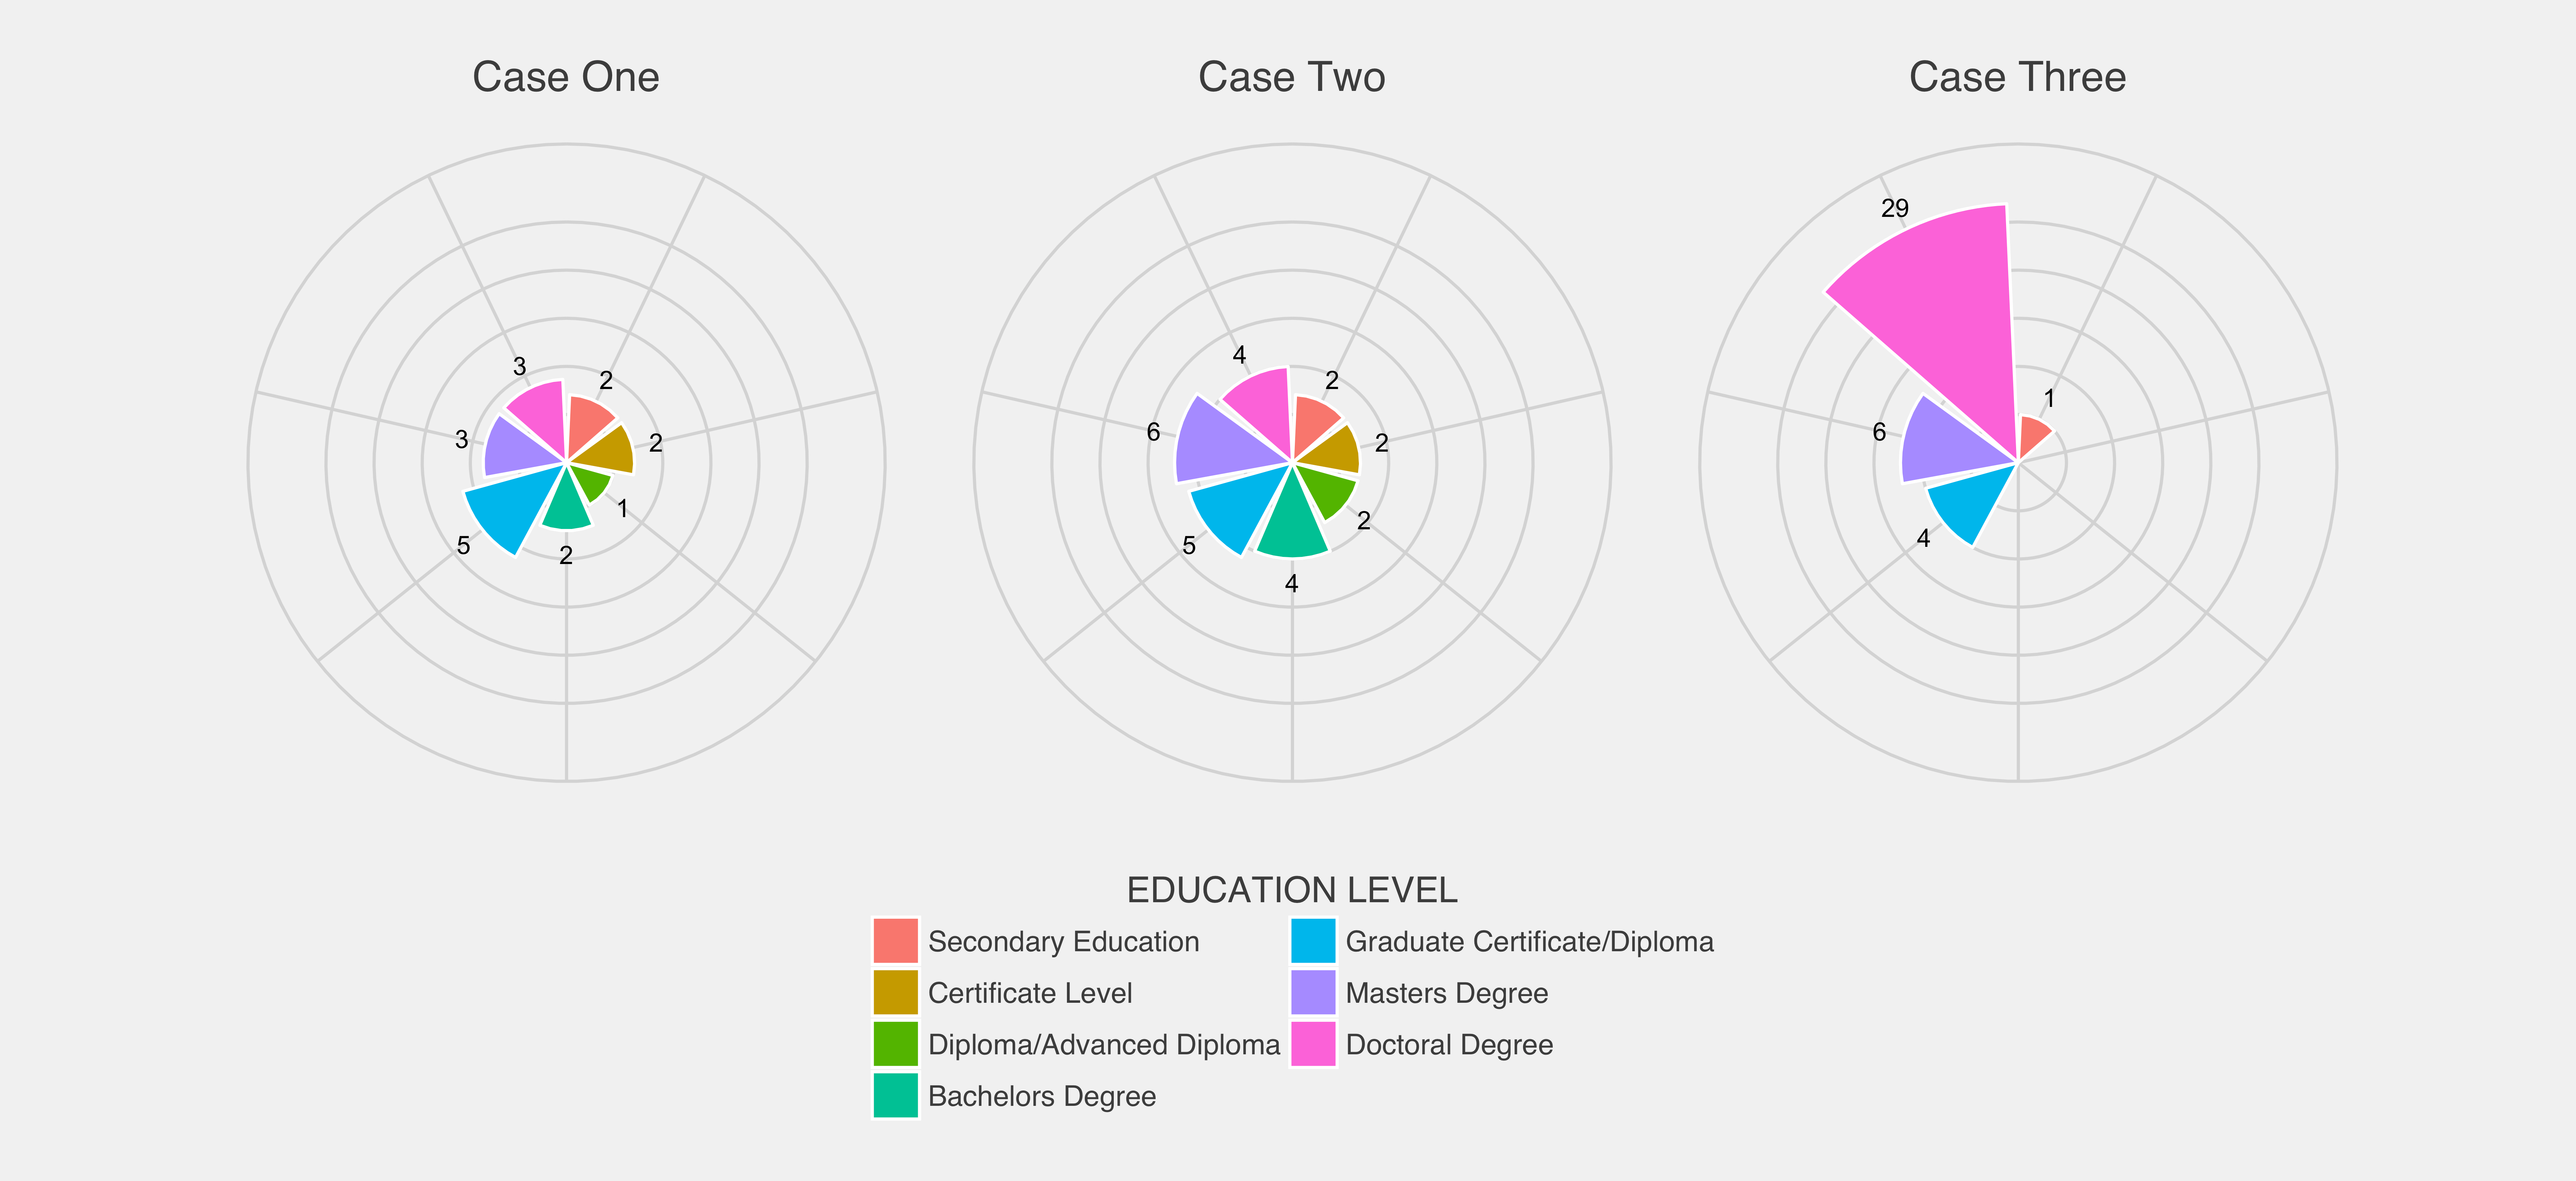
\includegraphics[width=1\linewidth]{Images/ed_level.png}
        \caption{Level of education}
        \label{fig:edlevel}
    \end{subfigure} \medskip
    
    \begin{subfigure}[b]{1\textwidth}
        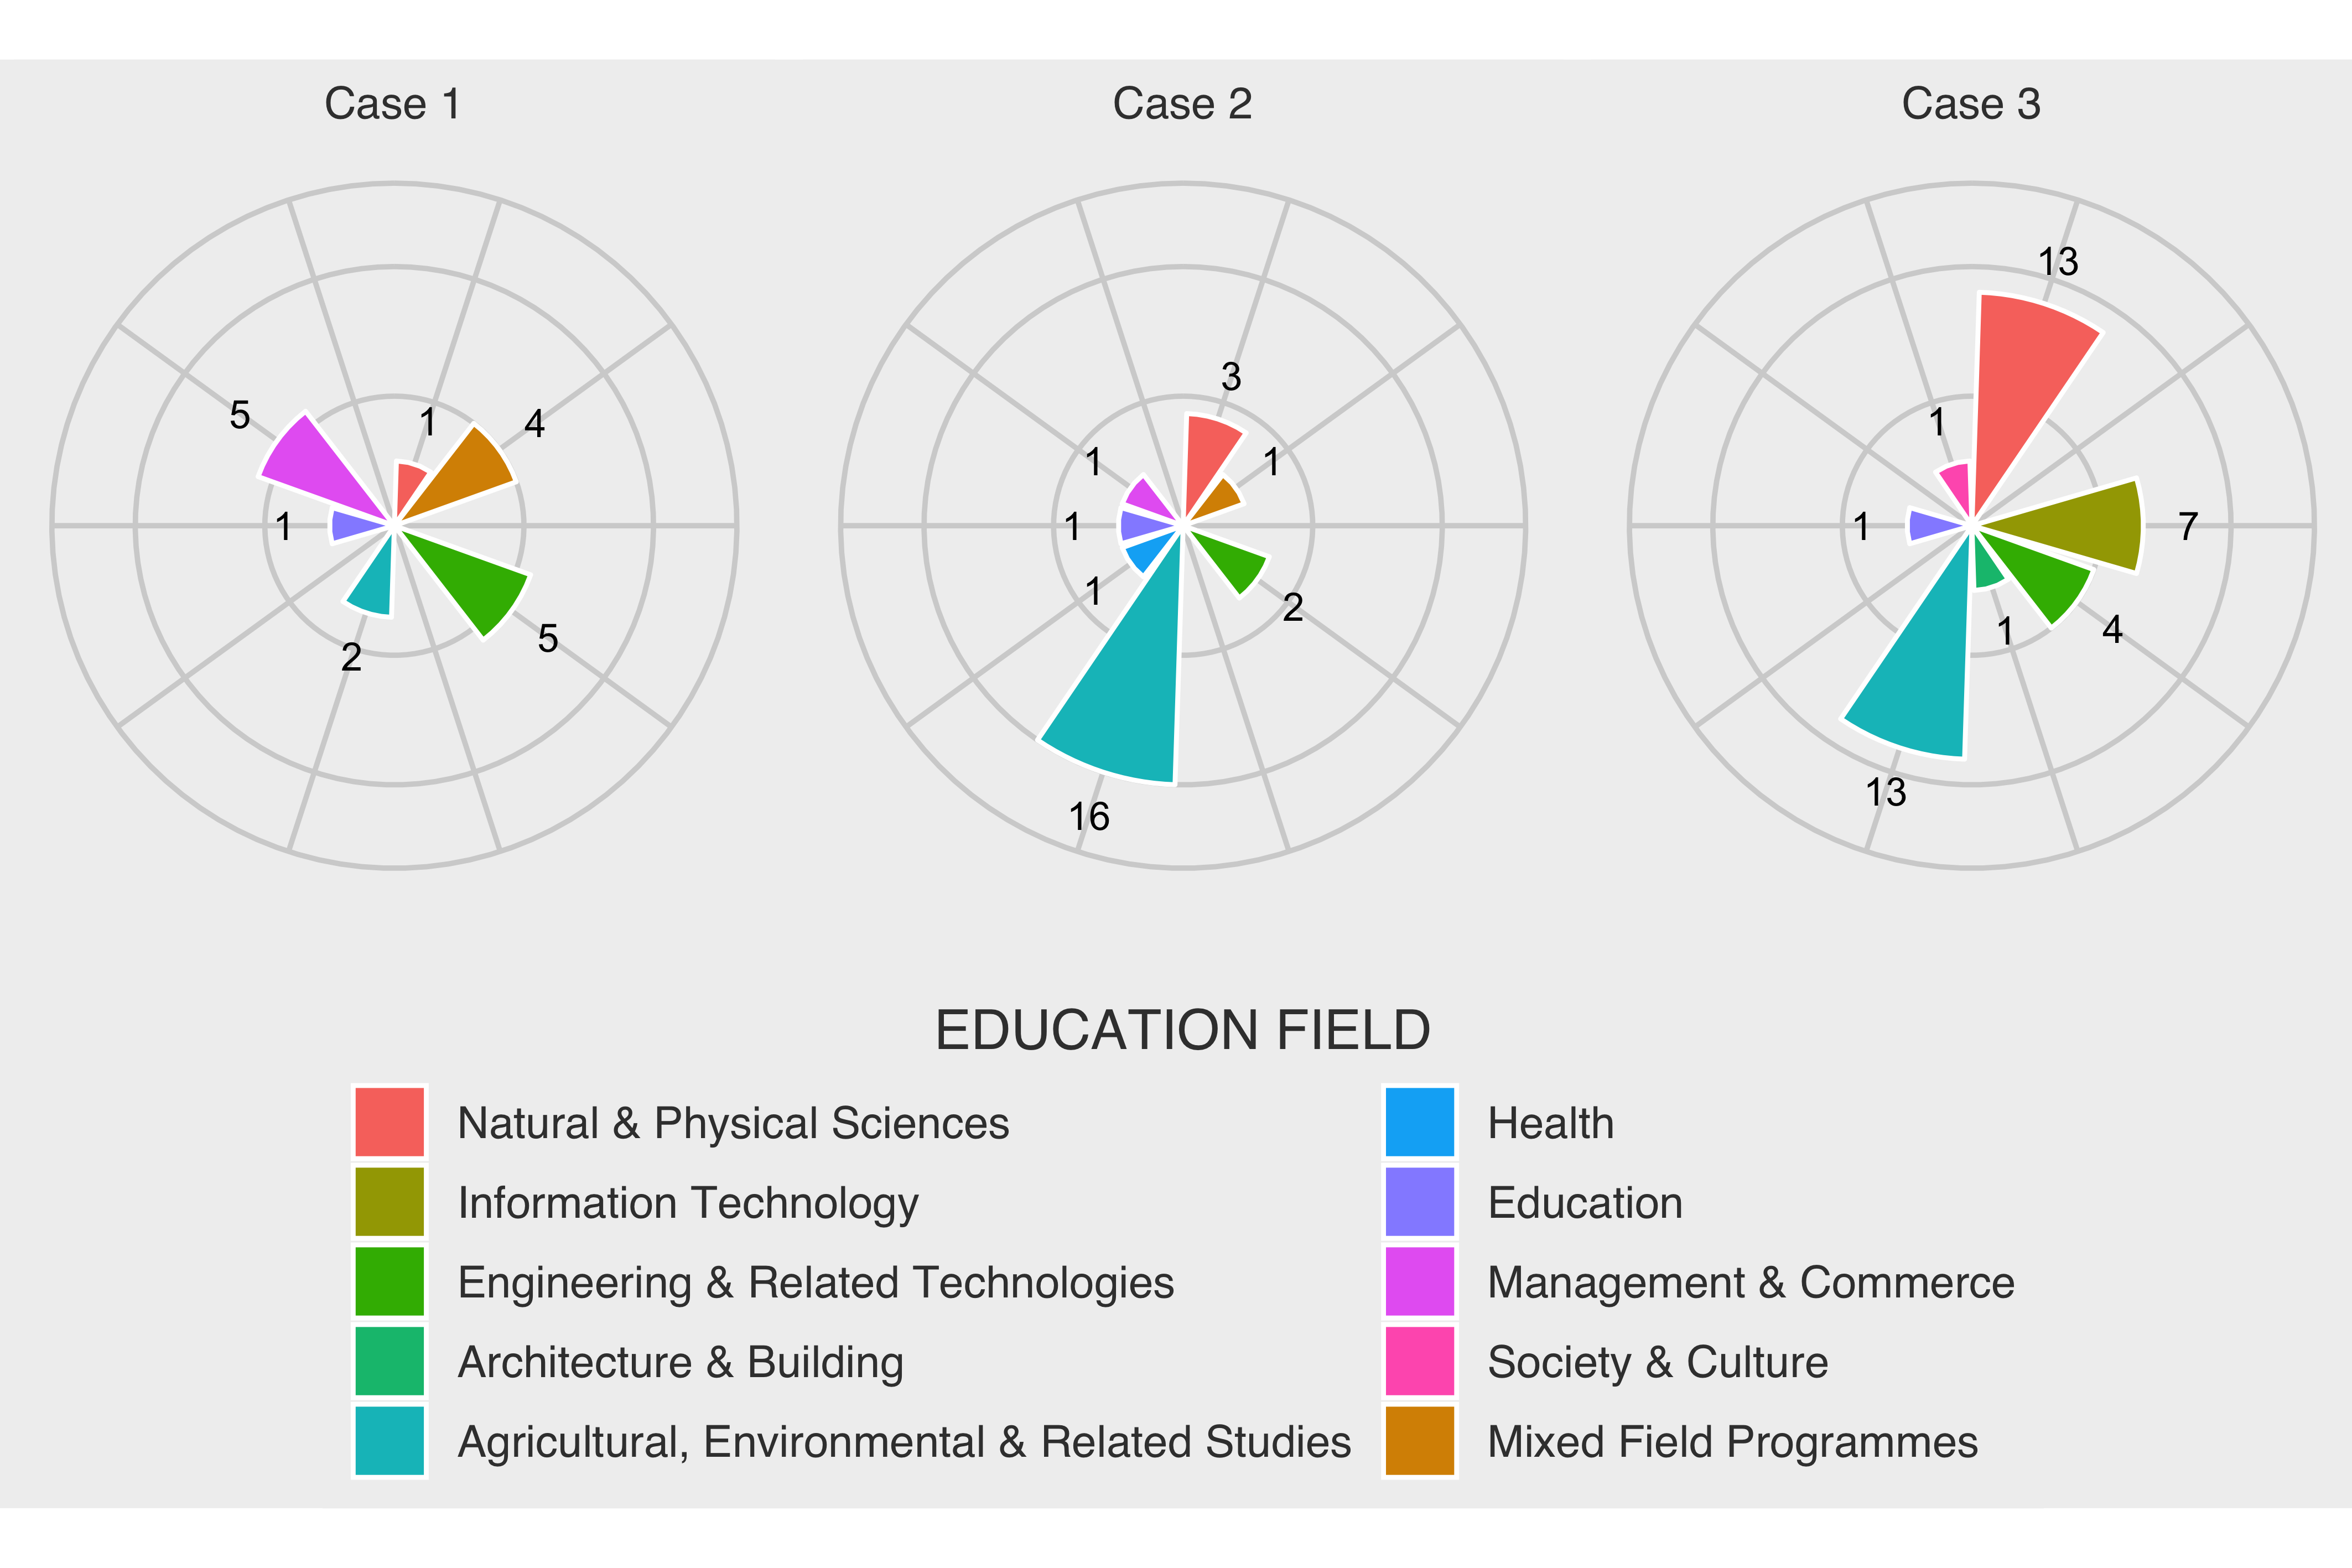
\includegraphics[width=1\linewidth]{Images/ed_field.png}
        \caption{Educational background}
        \label{fig:edfield}
    \end{subfigure} \medskip
 
    \begin{subfigure}[b]{1\textwidth}
        \includegraphics[width=1\linewidth]{Images/age_experience.png}
        \caption{Age and experience}
        \label{fig:years}
    \end{subfigure}
    \caption{Demographic information for each case}\label{fig:demographics}
\end{figure}

\begin{landscape}
    \begin{figure}
    \centering
    \begin{subfigure}[b]{0.5\textwidth}
        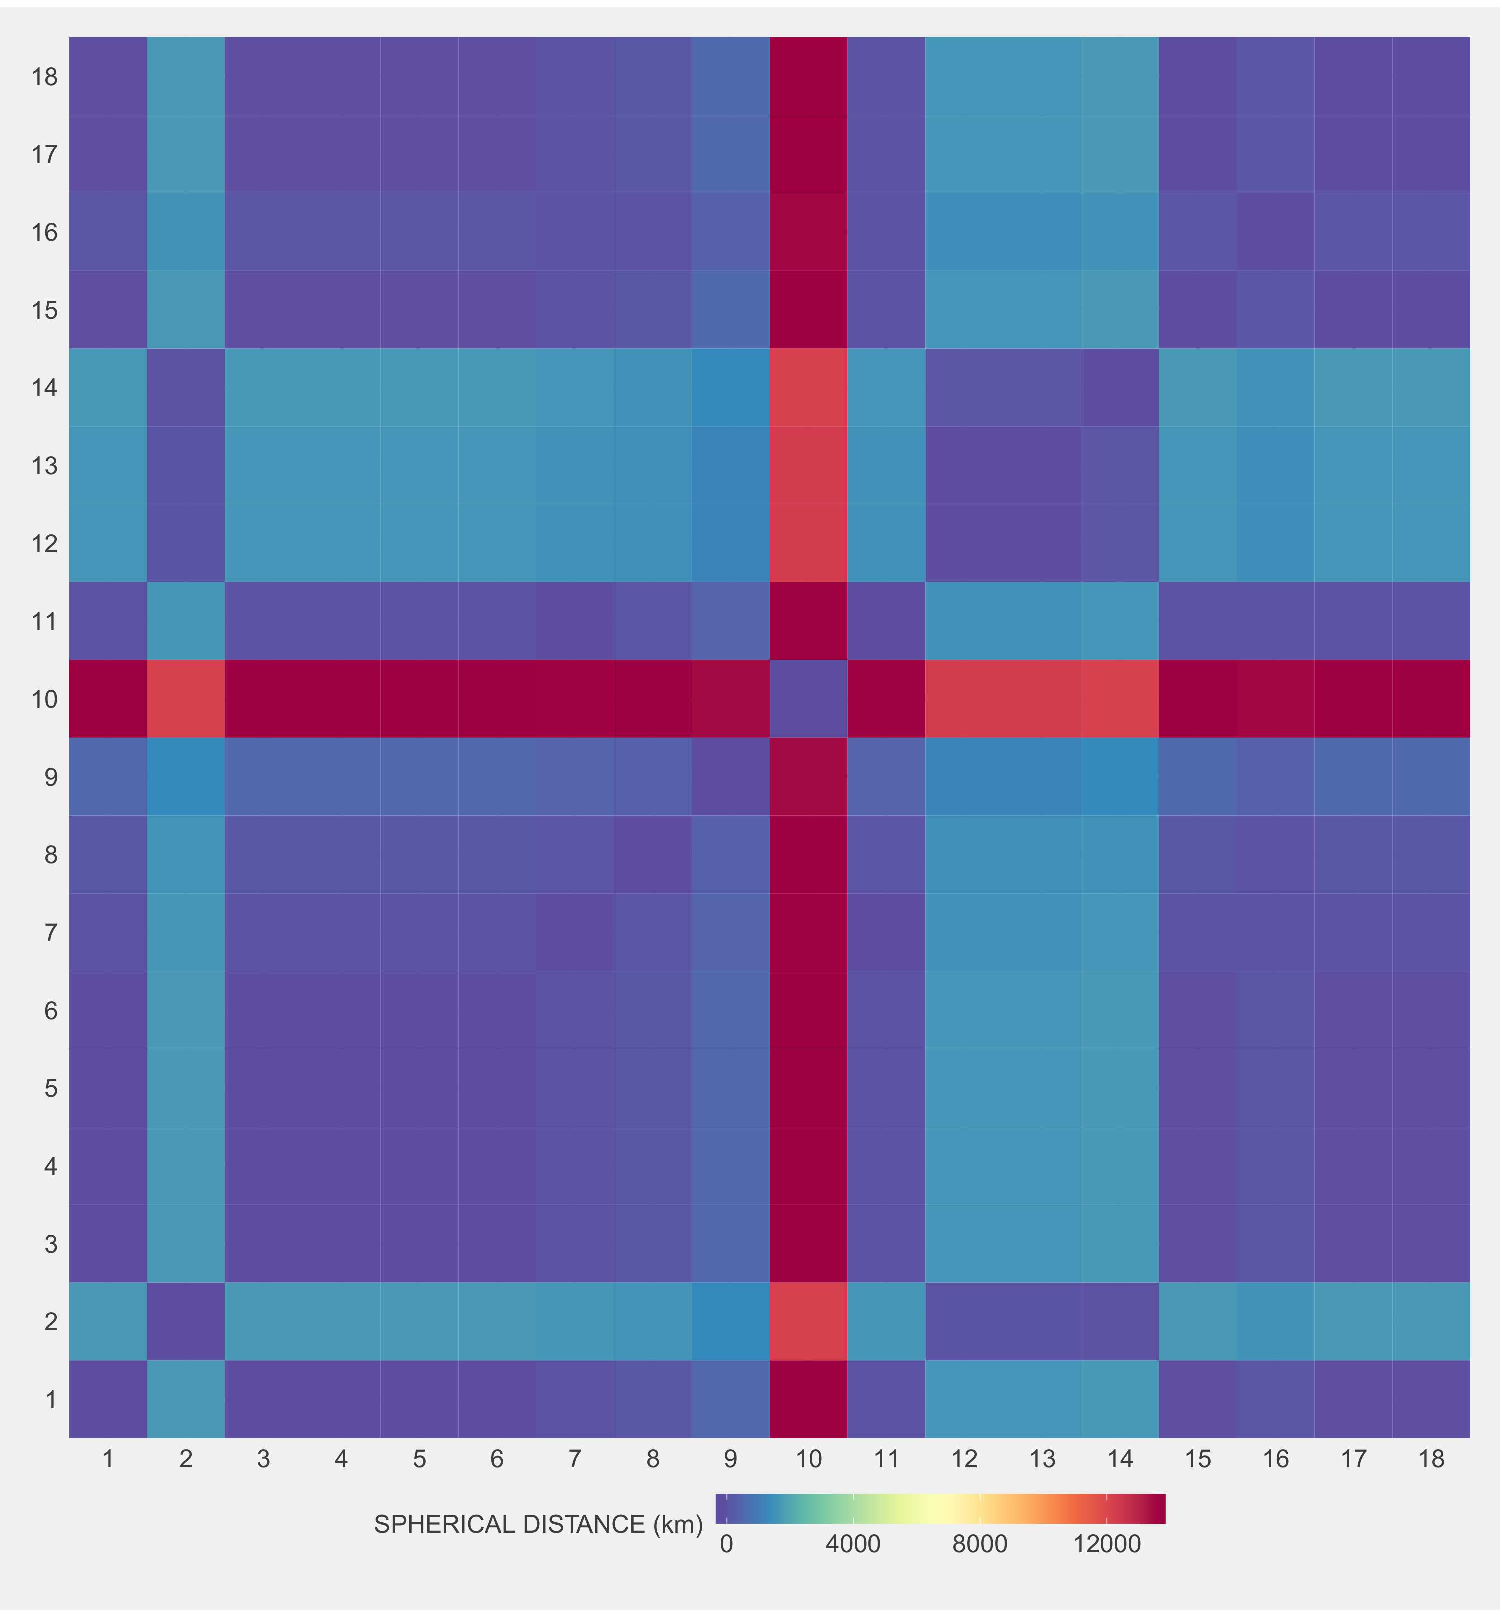
\includegraphics[width=0.9\linewidth]{Images/sph_distance_case1-eps-converted-to.pdf}
        \caption{Case One}
        \label{fig:proximity_c1}
    \end{subfigure} 
    \qquad
    \begin{subfigure}[b]{0.5\textwidth}
        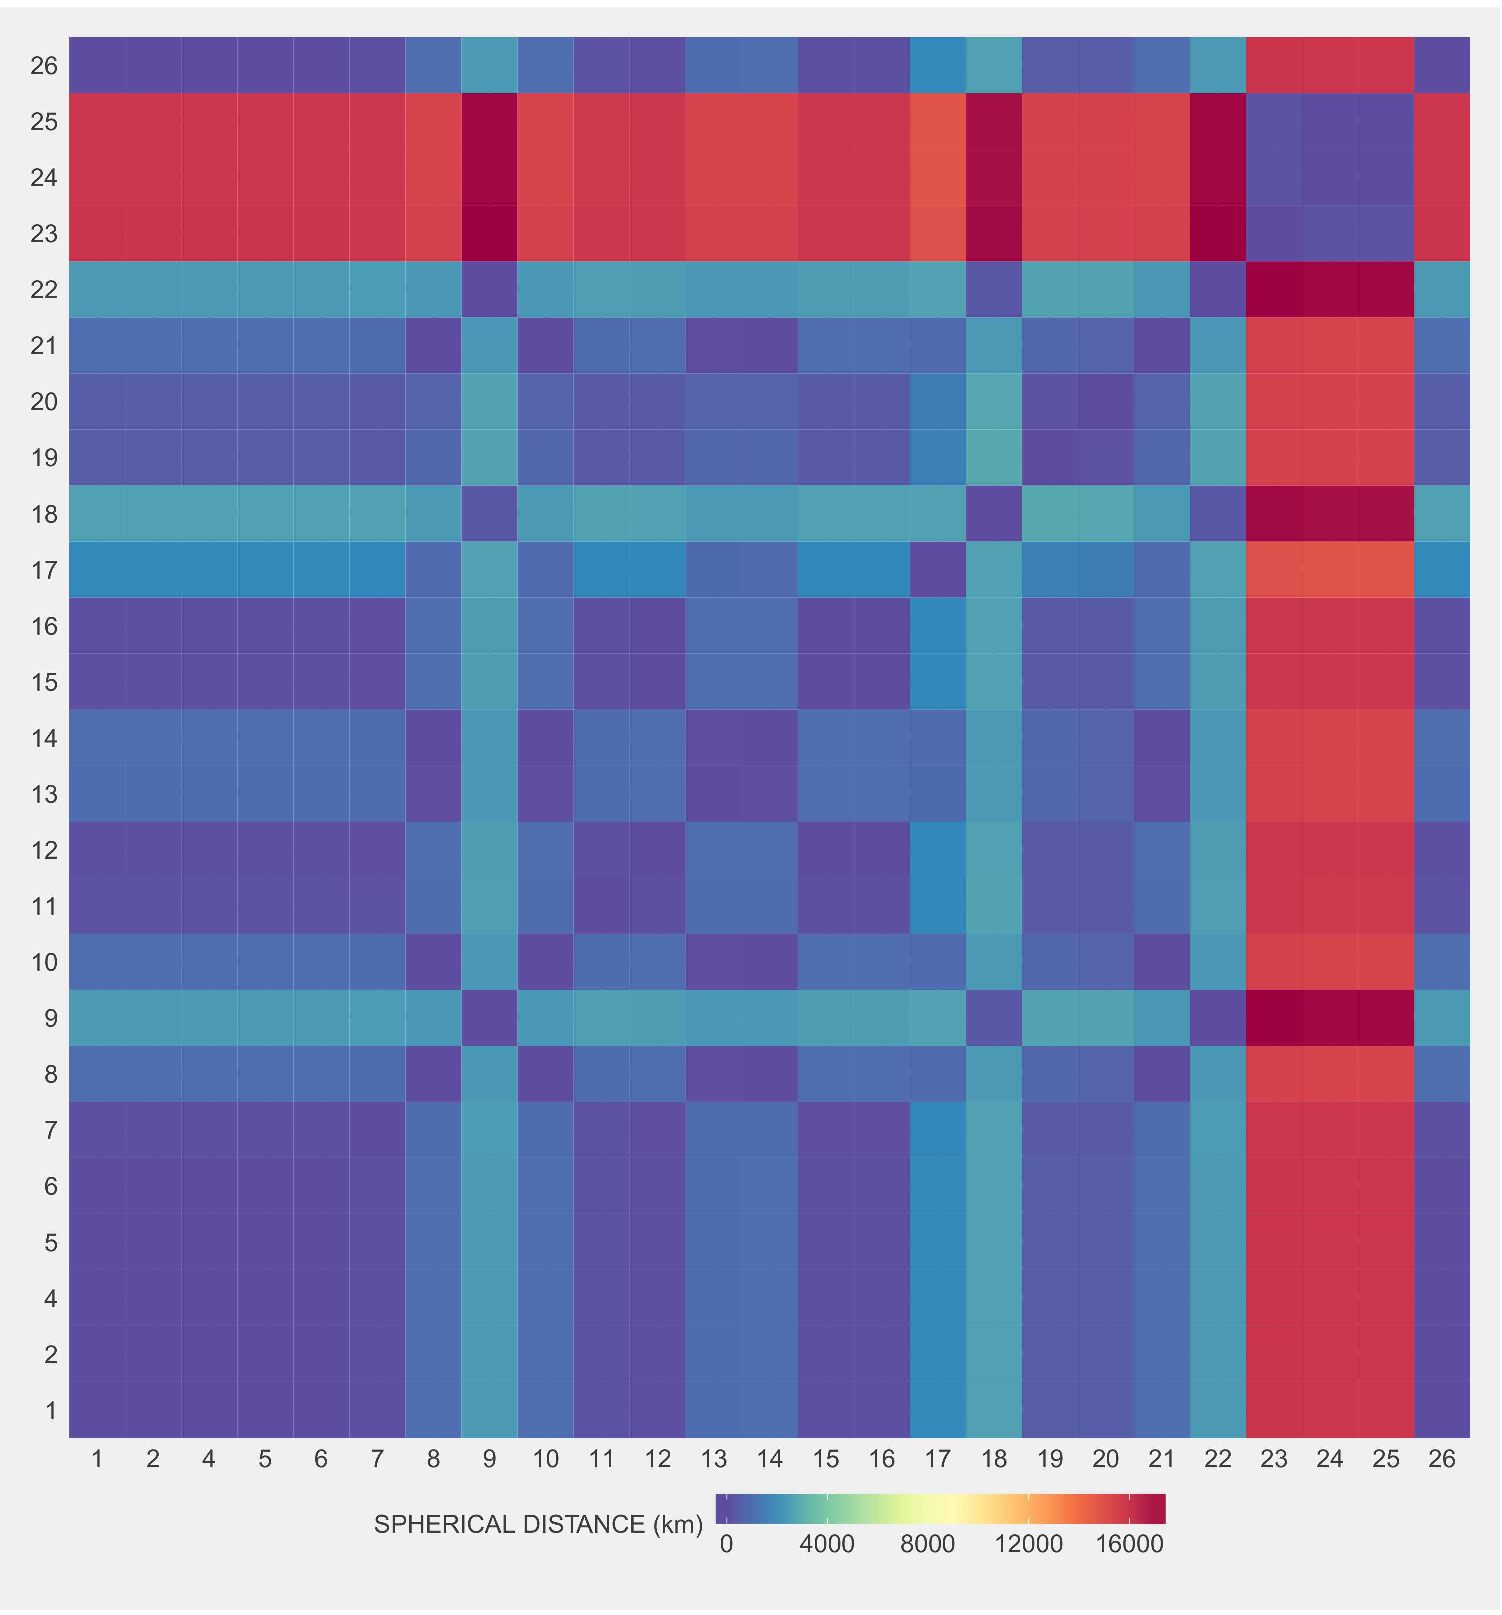
\includegraphics[width=0.9\linewidth]{sph_distance_case2-eps-converted-to.pdf}
        \caption{Case Two}
        \label{fig:proximity_c2}
    \end{subfigure}
    \qquad
    \begin{subfigure}[b]{0.5\textwidth}
        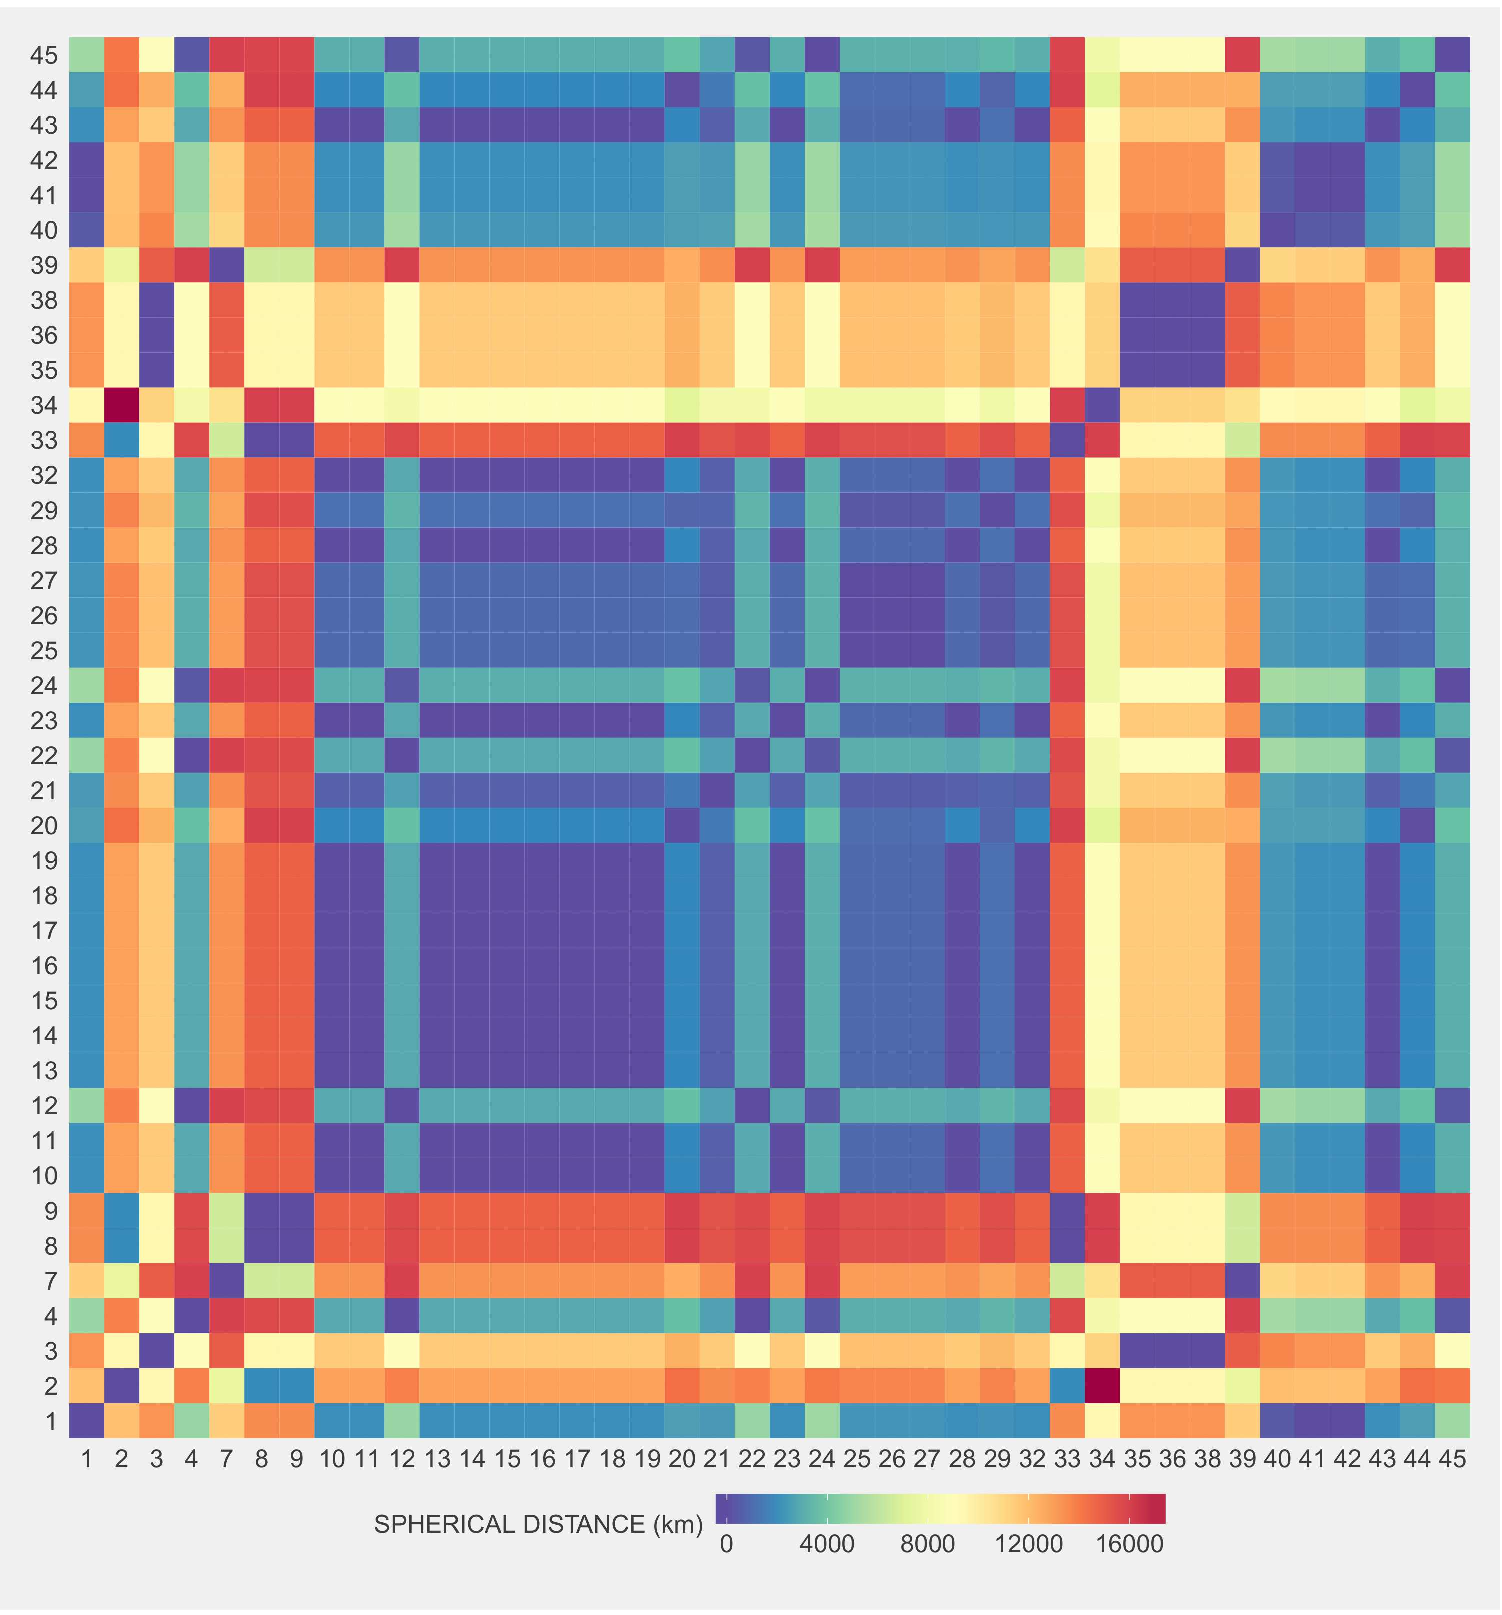
\includegraphics[width=0.9\linewidth]{Images/sph_distance_case3-eps-converted-to.pdf}
        \caption{Case Three}
        \label{proximity_c3}
    \end{subfigure}
    \caption{Distance matrices depicting the geographic separation, expressed as spherical distance, between actors}
    \label{fig:spherical}
\end{figure}
\end{landscape}

\subsection{Open innovation processes}

Case One is about \enquote{Herbs \& More} using external know-how and expertise to improve internal product handling processes. The innovation process is controlled by \enquote{Herbs \& More}. Case One is an example of \enquote{inbound open innovation}. \enquote{Dairy Tech} and \enquote{Smith \& Son} have joint control of the innovation process in Case Two. Both parties were learning from each other as they implemented a robotic dairy system to support voluntary milking. Case Two is an example of \enquote{coupled open innovation}. \enquote{National Research} were the instigator of the global partnership for honeybee research. They determined what technology had to be used and who could use it. \enquote{National Research} also provided the knowledge how to install and use the technology. Case Three is a good example of outbound open innovation. \medskip

Regarding case risk profiles, Case One had low exposure to financial and technological risk. The cold chain initiative may be regarded as an exercise in continuous improvement. Business operations at \enquote{Herbs \& More} were not dependent on the outcomes of the cold chain innovation initiative. This was not the case in Case Two, where both \enquote{Dairy Tech} or \enquote{Smith \& Sons} were exposed to considerable financial and technological risk. A poor outcome would also have damaged the market reputation of \enquote{Dairy Tech}. While Case Three had low exposure to financial risk, there was moderate technological risk. Failing to deliver on the promise of revolutionising honeybee research did expose \enquote{National Research} to considerable reputational risk. \medskip 

\subsection{Type of innovation}

Figure \ref{fig:innovation_type} depicts ten types of innovation across three broad categories. The first category, \enquote{configuration}, refers to innovations affecting the innermost workings of an enterprise and its business systems. It includes innovations relating to the profit model, strategic partnerships (networks), organisational structure, and internal processes. The second category, \enquote{offering}, refers to innovations relating to products and services provided by the enterprise, while the third category, \enquote{experience}, relates to customer-facing elements of an enterprise and its business system \citep{keeley2013ten}. Case One may be describes as an example of network, process, and product performance innovation, with process innovation being the dominant type. Case Two involves network, process, product performance and, most importantly, product system innovation. Case Three is an example of network and product system innovation. \medskip    

\begin{figure}
	\centering
	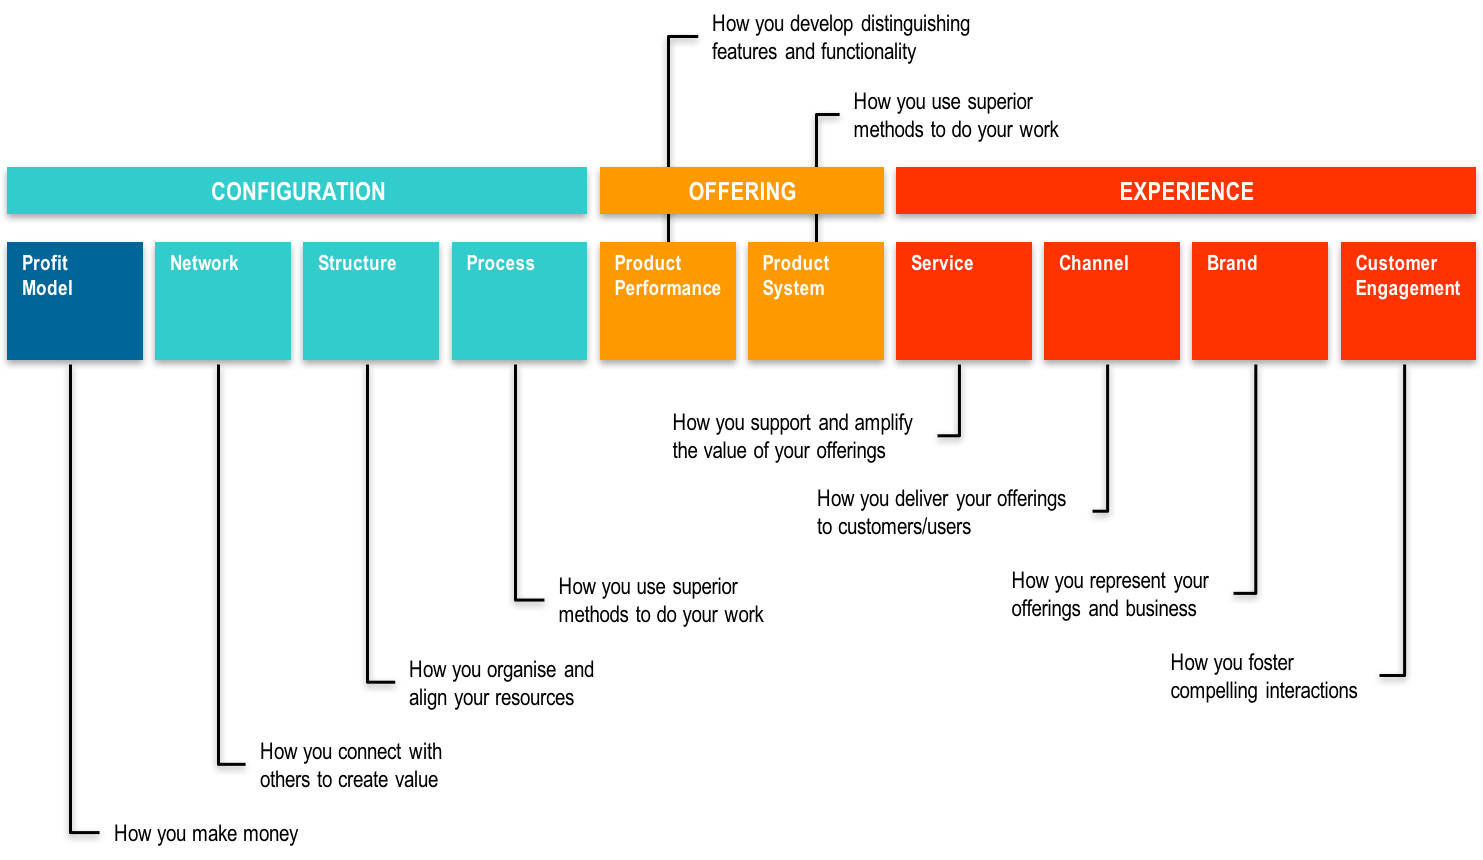
\includegraphics[width=1.0\linewidth]{Images/innovation_types.png}
	\caption{Types of innovation. From \citep{keeley2013ten}}.
	\label{fig:innovation_type}
\end{figure}

Table \ref{degree} refers to different degrees or intensities of innovation and what these mean in terms of technical change and economic impact \citep{coccia2005measuring}. Using this classification system, Case One can be categorised as a second-degree innovation activity with a mild level of innovation intensity and low economic impact. Descriptive terms such as \enquote{continuous}, \enquote{improvements}, \enquote{incremental}, and \enquote{minor} reflect the nature of innovation in Case One. Terms such as \enquote{breakthrough}, \enquote{radical}, \enquote{technology push} capture the essence of Case Two, which is categorised as a fifth-degree type innovation activity with a strong level of innovation intensity and medium economic impact. Case Three is categorised as a third- or fourth-degree innovation activity with a moderate to intermediate level of innovation intensity and low economic impact. Descriptors such as \enquote{major}, \enquote{really new}, \enquote{niche creation} are apt for Case Three.\medskip

\begin{table}[]
\centering
\caption{Classification of technical change. Based on \citet{coccia2005measuring}.}
\label{degree}
\begin{adjustbox}{width=\textwidth}
\begin{tabular}{@{}cccl@{}}
\toprule
Economic impact & Innovation degree & Innovation intensity & \multicolumn{1}{c}{Descriptive terms} \\ \midrule
\multirow{3}{*}[-5em]{Low} & 1 & Lightest & \begin{tabular}[c]{@{}l@{}}Micro-incremental \citep{coccia2005measuring} \\ Unrecorded \citep{freeman1994economics} \end{tabular} \\ \cline{3-4}
 & 2 & Mild & \begin{tabular}[c]{@{}l@{}}Continuous \citep{freeman1982unemployment} \\ Improvements \citep{mensch1979stalemate} \\ Incremental \citep{freeman1982unemployment} \\ Market pull \citep{dosi1988sources} \\ Minor \citep{henderson1990architectural} \\ Regular \citep{abernathy1985innovation} \end{tabular} \\ \cline{2-4}
 & 3 & Moderate & \begin{tabular}[c]{@{}l@{}}Major \citep{o2008major} \\ Market breakthrough \citep{chandy2000incumbent} \\ Modular \citep{henderson1990architectural} \\  Non-drastic \citep{arrow1962welfare} \\ Really new \citep{garcia2003critical} \end{tabular} \\ \midrule
\multirow{2}{*}[-4em]{Medium} & 4 & Intermediate & \begin{tabular}[c]{@{}l@{}}Micro-radical \citep{durand1992dual} \\ Niche creation \citep{abernathy1985innovation} \\ Non-drastic \citep{arrow1962welfare} \\ Technological breakthrough \citep{chandy2000incumbent} \end{tabular} \\ \cline{3-4}
 & 5 & Strong & \begin{tabular}[c]{@{}l@{}}Architectural \citep{abernathy1985innovation} \\ Basic innovation \citep{mensch1979stalemate} \\ Breakthrough \citep{tidd1995development} \\ Discontinuous \citep{birkinshaw2007finding} \\ Drastic \citep{arrow1962welfare} \\ Fundamental \citep{mensch1979stalemate} \\ Radical \citep{freeman1982unemployment} \\ Technology push \citep{dosi1988sources} \end{tabular} \\ \midrule
\multirow{2}{*}[-1em]{High} & 6 & Very strong & \begin{tabular}[c]{@{}l@{}}New technological systems \citep{freeman1982unemployment} \\ Innovation systems \citep{sahal1981patterns} \end{tabular} \\ \cline{3-4}
 & 7 & Revolutionary  & \begin{tabular}[c]{@{}l@{}}Change of technology paradigms \citep{dosi1982technological} \\ Revolutionary \citep{abernathy1985innovation} \\ Technological revolutions \citep{freeman1982unemployment} \end{tabular} \\ \bottomrule
\end{tabular}
\end{adjustbox}
\end{table}

\subsection{Demographic make-up}

Figure \ref{fig:edlevel} indicates participants in both Case One and Case Two have a similar range of education level. Most participants in these two cases have some form of post-graduate qualification. Case Three is heavily dominated by people with doctoral level qualifications. This is not surprising, given most participants work either at universities or in government research agencies. Figure \ref{fig:edfield} shows the people in Case One are most likely to have an educational background in either management and commerce, engineering, or mixed field programmes. There is no dominant educational background, unlike in Case Two, which heavily dominated by people with a background in agricultural or environmental studies. The dominant educational backgrounds in Case Three are agriculture and environmental studies and natural and physical sciences. This suggest that Case One and Three are more multidisciplinary than Case Two.\medskip

In terms of age, relevant work experience, and job tenure, the median age of participants in all three cases falls between 40 and 50 years. People in Case Two and Case Three have similar levels of relevant work experience.  Participants in Case One have slightly lower work experience compared to those in the other two cases. Job tenure is highest in Case Two. Case Three is dominated by people with relatively low job tenure. Job tenure is relatively low in Case One (\enquote{Herbs \& More} is a relatively young enterprise. The research group at \enquote{State University} was only recently established). The level of work experience and job tenure is highest in Case Two. This suggests that tacit knowledge, which is borne from experience, is more likely to feature in Case Two than in Case One or Case Three. \medskip 

% geographic separation.

Table \ref{cases} summarises the key characteristics of each case. The next chapter (Chapter 6) reports on how individual attributes such as level of personal motivation, education level, work location, and job experience shape tacit knowledge sharing relations in each open innovation partnership. \medskip

\begin{table}
\centering
\caption{Characteristic features of each case}
\label{cases}
\begin{adjustbox}{width=\textwidth}
\begin{tabular}{@{}cllcccc@{}}
\toprule
Case & \multicolumn{1}{c}{Description} & \multicolumn{1}{c}{Innovation Challenge} & \begin{tabular}{@{}c@{}}Type of \\ open innovation \end{tabular} & \begin{tabular}{@{}c@{}}Project \\ stage \end{tabular} & \begin{tabular}{@{}c@{}}Partner \\ organisations \end{tabular} & \begin{tabular}{@{}c@{}}Individual \\ participants \end{tabular} \\ \midrule
1 & Cold chain innovation & \begin{tabular}[t]{@{}l@{}}Extend shelf-life of green-leaf vegetables\end{tabular} & Inbound & \begin{tabular}[t]{@{}c@{}}Early \\ execution \end{tabular} & 7 & 18 \\
2 & Farm system innovation & \begin{tabular}[t]{@{}l@{}}Implement robotic dairy system based \\ on voluntary cow traffic \end{tabular} & Coupled & Closure & 8 & 25 \\
3 & \begin{tabular}[t]{@{}l@{}}Innovative global research \\ partnership \end{tabular} & \begin{tabular}[t]{@{}l@{}} Develop near real-time web-based data \\ analysis system for tracking bee \\ movements in and out of hives \end{tabular} & Outbound & \begin{tabular}[t]{@{}c@{}}Very \\ early \\ execution \end{tabular} & 14 & 40 \\ \bottomrule
\end{tabular}
\end{adjustbox}
\end{table}